\newpage
\section[Functions of Several Variables]{\hyperlink{toc}{Functions of Several Variables}}

\subsection{Banach Fixed Point Theorem}
\noindent Our goal in this chapter will be to work up to the Inverse Function Theorem. This chapter in Rudin begins by covering the necessary results in linear algebra; we will assume this has been covered in a prior course, so we will omit discussion of items 9.1-9.9. However, these can be read for a refresher of the material.

We will start off this chapter with discussion of the Banach fixed point theorem (also known as the Contraction principle), as it is independent of the rest of the chapter's content. It will be used in the proof of the inverse function theorem, but also applies in a more general setting.

\setcounter{rudin}{21}

\begin{definition}{Contractions}{9.22}
    Let $(X, d)$ be a metric space. Suppose there exists $c < 1$ such that the map $\phi: X \mapsto X$ satisfies $d(\phi(x), \phi(y)) \leq cd(x, y)$ for all $x, y \in X$ (that is, the images of $x, y$ are closer by a factor $c$ compared to the original $x, y$). Then, we call $\phi$ a \textbf{contraction} of $X$ into $X$.
\end{definition}
\begin{nlemma}{}{}
    Every contraction $\phi: X \mapsto X$ is uniformly continuous.
\end{nlemma}
\begin{nproof}
    Take $\delta = \frac{\e}{c}$ in the definition of uniform continuity. \qed
\end{nproof}

\begin{theorem}{Banach Fixed Point Theorem/Contraction Mapping Theorem}{9.23}
    Let $(X, d)$ be a complete metric space, and suppose $\phi: X \mapsto X$ is a contraction. Then, there exists a unique $x \in X$ such that $\phi(x) = x$. We call this x a \emph{fixed point}. 
\end{theorem}
\noindent The proof of the above theorem gives an algorithm to find $x$ which converges exponentially fast.

\begin{figure}[htbp]
    \centering
    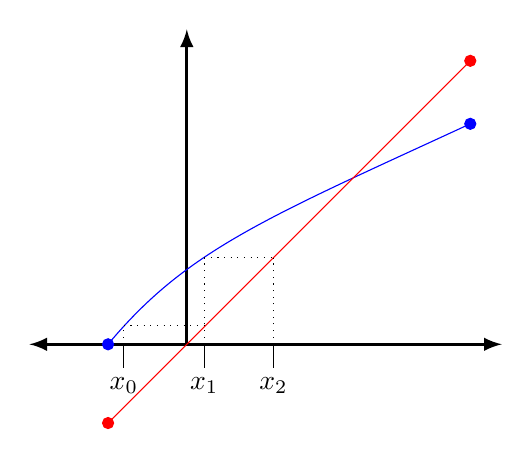
\begin{tikzpicture}[scale=2]
        \draw[-latex, very thick] (0, 0) -- (2, 0);
        \draw[-latex, very thick] (0, 0) -- (0, 2);
        \draw[-latex, very thick] (0, 0) -- (-1, 0);
        \draw[blue] (-0.5, 0) .. controls (0, 0.6) and (0.5, 0.8 ).. (1.8, 1.4);
        \draw[fill = blue, draw = blue] (-0.5, 0) circle (1pt);
        \draw[fill = blue, draw = blue] (1.8, 1.4) circle (1pt);
        \draw[red] (-0.5, -0.5) -- (1.8, 1.8);
        \draw[fill = red, draw = red] (-0.5, -0.5) circle (1pt);
        \draw[fill = red, draw = red] (1.8, 1.8) circle (1pt);
        \draw[] (-0.4, 0) -- (-0.4, -0.15);
        \node[below] at (-0.4, -0.15) {$x_0$};
        \draw[dotted] (-0.4, 0) -- (-0.4, 0.12);
        \draw[dotted] (-0.4, 0.12) -- (0.13, 0.12);
        \draw[dotted] (0.11, 0) -- (0.11, 0.55);
        \draw[] (0.11, 0) -- (0.11, -0.15);
        \node[below] at (0.11, -0.15) {$x_1$};
        \draw[dotted] (0.11, 0.55) -- (0.55, 0.55);
        \draw[dotted] (0.55, 0) -- (0.55, 0.55);
        \draw[] (0.55, 0) -- (0.55, -0.15);
        \node[below] at (0.55, -0.15) {$x_2$};
    \end{tikzpicture}

    \caption{Visualization of the algorithm for finding the fixed point $x$ in Theorem \ref{thm:9.23} for the case where $X = \RR$. The fact that $\phi$ is a contraction makes it such that it has slope less than $1$. The fixed point is the point of intersection between $y = x$ and $y = \phi(x)$. The iterative algorithm sketched above gives an exponentially fast way of finding this point of intersection, by iteratively applying $\phi$ to the initial guess $x_0$.}
    \label{fig59}
\end{figure}

\begin{nproof}
    We first show uniqueness. If $\phi(x) = x$ and $\phi(y) = y$, then $d(\phi(x), \phi(y)) \leq cd(x, y)$. But since $c < 1$, $d(x, y) \leq cd(x, y)$ is only satisfied if $d(x, y) = 0$. Hence, $x = y$ and the fixed point is unique.

    We next show existence. Given $x_0 \in X$, let $x_1 = \phi(x_0)$, $x_2 = \phi(x_1) = \phi\circ \phi(x_0)$, $x_3 = \phi(x_2) = \phi\circ\phi\circ\phi(x_0)$ and so on, with $x_{n+1} = \phi(x_n) = \phi \circ \ldots \circ \phi(x_0)$ with the composition carried out $n+1$ times. The goal is to show this sequence is Cauchy, and has a limit which is a fixed point. We then have that $d(x_{n+1}, x_{n+2}) = d(\phi(x_n), \phi(x_{n+1})) \leq cd(x_{n+1}, x_n)$, so by induction, it follows that $d(x_{n+1}, x_n) \leq c^nd(x_1, x_0)$. Hence, for $n > m$ we have that:
    \begin{align*}
        d(x_n, x_m) &\leq \sum_{i=m+1}^n d(x_i, x_{i-1}) & \text{(Triangle Inequality)}
        \\ &\leq \sum_{i=m+1}^n c^{i-1}d(x_1, x_0)
        \\ &\leq \sum_{i=m+1}^\infty c^{i-1}d(x_1, x_0)
        \\ &= \frac{c^m}{1-c}d(x_1, x_0) & \text{(Convergent Geometric Series)}
    \end{align*}
    $c^m$ can be as small as we like by taking sufficiently large $m$, so $\set{x_n}$ is Cauchy, and by the completeness of $X$, $x_n \rightarrow x$ for some $x$. Since $\phi$ is a contraction, it is (uniformly) continuous by the above Lemma, and since $x_n \rightarrow x$, we have that $\phi(x_n) \rightarrow \phi(x)$, and hence:
    \begin{align*}
        \phi(x) = \linf \phi(x_n) = \linf x_{n+1} = x.
    \end{align*}
    This shows that $x$ is the desired fixed point. \qed
\end{nproof}

\subsection{Differentiation of Functions of Several Variables}

\subsection{The Inverse Function Theorem}

